\documentclass[tikz,border=2pt]{standalone}
\usepackage{amsmath}
\usepackage{pgfplots}
\pgfplotsset{compat=1.18}
\usetikzlibrary{arrows.meta}
\begin{document}
% Solutions x(t) = 1/2 + C e^{-2t} of x' + 2x = 1 for C = 1, -1/2, -1: every solution tends to the
% equilibrium q/p = 1/2; the initial value problem x(0) = 0 picks C = -1/2, x(t) = (1 - e^{-2t})/2.
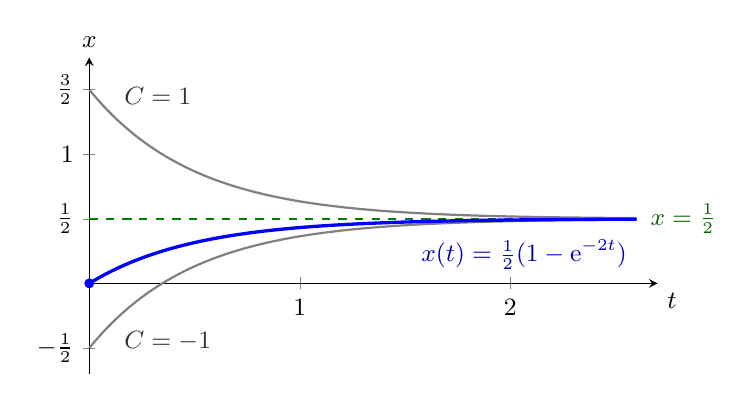
\begin{tikzpicture}[font=\small, >={Latex[length=2mm]}]
  \begin{axis}[
    axis lines=middle,
    xmin=0, xmax=2.7, ymin=-0.7, ymax=1.75,
    xtick={1,2}, ytick={-0.5,0.5,1,1.5},
    yticklabels={$-\tfrac{1}{2}$,$\tfrac{1}{2}$,$1$,$\tfrac{3}{2}$},
    xlabel={$t$}, ylabel={$x$},
    xlabel style={anchor=north west}, ylabel style={anchor=south},
    samples=120, clip=false,
    width=8.8cm, height=5.6cm
  ]
    \addplot[green!50!black, thick, dashed, domain=0:2.6] {0.5};
    \addplot[gray, thick, domain=0:2.6] {0.5+exp(-2*x)};
    \addplot[gray, thick, domain=0:2.6] {0.5-exp(-2*x)};
    \addplot[blue, very thick, domain=0:2.6] {0.5-0.5*exp(-2*x)};
    \fill[blue] (axis cs:0,0) circle (1.8pt);
    \node[gray!40!black, anchor=west] at (axis cs:0.12,1.45) {$C=1$};
    \node[gray!40!black, anchor=west] at (axis cs:0.12,-0.45) {$C=-1$};
    \node[blue!70!black, anchor=north east] at (axis cs:2.6,0.41) {$x(t)=\tfrac{1}{2}(1-\mathrm{e}^{-2t})$};
    \node[green!40!black, anchor=west] at (axis cs:2.62,0.5) {$x=\tfrac{1}{2}$};
  \end{axis}
\end{tikzpicture}
\end{document}
